\def\year{2017}\relax
%File: formatting-instruction.tex
%\documentclass[letterpaper]{article}
\documentclass[letterpaper]{article}
\usepackage{geometry}
\geometry{left=2.5cm,right=2.5cm,top=2.5cm,bottom=2.5cm}
%\usepackage{aaai17}
\usepackage{amsmath}
\usepackage{amsthm}
\usepackage{times}
\usepackage{helvet}
\usepackage{courier}
\usepackage{graphicx}
\usepackage{subfigure}
\usepackage{mdwmath}
\usepackage{mdwtab}
\usepackage{amssymb}
\usepackage{booktabs}
\usepackage{algorithm}
\usepackage{pifont}
%\usepackage[noend]{algpseudocode}
\usepackage{algpseudocode}
\usepackage{balance}
\usepackage{bm}
\usepackage{ulem}
\usepackage{array}
\usepackage{balance}
\usepackage{multirow}
\usepackage{multicol}
\usepackage{threeparttable}
\frenchspacing
%\setlength{\pdfpagewidth}{8.5in}
%\setlength{\pdfpageheight}{11in}
\usepackage[marginal]{footmisc}
\usepackage{extarrows}
\usepackage{natbib}
 \title{Speed Maintained SVRG}
\setcounter{secnumdepth}{0}  

%add the command initial
\algnewcommand\algorithmicInitial{\textbf{Initialize:}}
\algnewcommand\Initial{\item[\algorithmicInitial]}
\algnewcommand\algorithmicIterate{\textbf{Iterate:}}
\algnewcommand\Iterate{\item[\algorithmicIterate]}


 \begin{document} 
 \maketitle
 

 
 \begin{algorithm}[t]
 	\caption{Speed Maintained SVRG}
	\label{algorithm_SMSVRG}
	\begin{algorithmic}[1]
	\Require learning rate $\eta$, minimal epoch size $m_0$
	\Initial $\tilde{\omega}_0=\mathbf{0}$, k=0
	\State $\tilde{\mu} = \frac{1}{n}\sum\limits_{i=1}^{n}\nabla f_{i}(\tilde{\omega}_{0})$
	\For {$s=0, 1, ...$}
		\State $\omega_0 = \tilde{\omega}_s$
		%compute the full gradient 
		\For {$t=0, 1, ..., m_0$}
			\State Randomly pick $i_t\in\{1, 2, ..., n\}$
			\State $\omega_t = \omega_{t-1} - \eta(\nabla f_{i_t} - \nabla f_{i_t}(\tilde{\omega}_s)+\tilde{\mu})$
		\EndFor
		\State $\tilde{\omega}_{s+1} = \omega_{\frac{n}{2}}$
		
		\If{ $s>1$ and $\frac{\Vert  \tilde{\omega}_{s+1} - \tilde{\omega}_{s}  \Vert} 
			{\Vert  \tilde{\omega}_{s} - \tilde{\omega}_{s-1}  \Vert}  <
			\frac{\Vert \tilde{\omega}_{s} - \tilde{\omega}_{s-1}  \Vert } 
			{\Vert  \tilde{\omega}_{s-1} - \tilde{\omega}_{s-2}  \Vert}$}
		\State $\tilde{\mu} = \frac{1}{n}\sum\limits_{i=1}^{n}\nabla f_{i}(\tilde{\omega}_{s+1})$
		\EndIf	
	\EndFor
	\State \Return $\tilde{\omega}_{s+1}$
	\end{algorithmic}	
\end{algorithm}

 \section{Speed Maintained SVRG}
 In this section we describe a novel algorithm: Speed Maintained SVRG (\textsc{smSVRG}), which can set the appropriate iteration number in each epoch automatically and has superior convergence properties in our experiments. 
 
 Algorithm \ref{algorithm_SMSVRG} just requires two parameters: learning rate $\eta$, mini-epoch size $m_0$. There are two loops in \textsc{smSVRG}. In the outer loop(we call each outer iteration as an mini-epoch),  $m_0$ SGD iterations are computed. And then we compute the inequality 
 \begin{equation}
 \label{inequality_1}
 \frac{\Vert  \tilde{\omega}_{s+1} - \tilde{\omega}_{s}  \Vert} {\Vert  \tilde{\omega}_{s} - \tilde{\omega}_{s-1}  \Vert}  <\frac{\Vert \tilde{\omega}_{s} - \tilde{\omega}_{s-1}  \Vert } {\Vert  \tilde{\omega}_{s-1} - \tilde{\omega}_{s-2}  \Vert}
 \end{equation}
 If the inequality holds, we compute a snapshot of the full gradient and step into a new mini-epoch. Otherwise, a new mini-epoch begins directly. It is apparent that we cannot compute the inequality until we have finished two mini-epochs. Note mini-epoch is different from epoch in SVRG, thus we define one epoch as the group of all mini-epochs between two full gradient computations.
 
 In practical experiments, we modify the inequality as follows:
 \begin{equation}
 \label{inequality_2}
 \frac{\Vert  \tilde{\omega}_{s+1} - \tilde{\omega}_{s}  \Vert} {\Vert  \tilde{\omega}_{s} - \tilde{\omega}_{s-1}  \Vert}  <(\frac{\Vert \tilde{\omega}_{s} - \tilde{\omega}_{s-1}  \Vert } {\Vert  \tilde{\omega}_{s-k} - \tilde{\omega}_{s-k-1}  \Vert})^\frac{1}{k}
 \end{equation}
 which can reduce the errors incurred by variance and have a better performance than the former.
  
 
 \section{Numerical Experiments}
 \subsection{Experimental settings}
 In this section, we conduct some experiments to illustrate the efficiency of our proposed algorithm, i.e. \textsc{smSVRG}. We evaluate our algorithm on eight training datasets, which are public on the LIBSVM website\footnote{http://www.csie.ntu.edu.tw/$\sim$cjlin/libsvmtools/datasets/}. In our experiments, \textsc{sbSBRG} is applied for two standard machine learning tasks: $l2$-regularized logistic regression and $l2$-regularized ridge regression.
 
 The $l2$-regularized logistic regression task is conducted on the four datasets: ijcnn1, a9a, mushrooms, w8a. Since the label of each instance in these datasets is set to be 1 or -1, the loss function of $l2$-regularized logistic regression task is:
\begin{equation}
\label{logistic_reg}
\min\limits_\omega \frac{1}{n}\sum\limits_{i=1}^n \log(1+e^{-y_i \omega^\mathrm{T} x_i }) + \lambda \parallel \omega \parallel^2.
\end{equation}
The $l2$-regularized ridge regression task is conducted on the four datasets: abalone, cadata, cpusmall, space\_ga. The loss function of $l2$-regularized ridge regression task is:
\begin{equation}
\label{ridge_reg}
\min\limits_\omega \frac{1}{n}\sum\limits_{i=1}^n\left(\omega^{\mathrm{T}}x_i-y_i\right)^2 + \lambda \parallel \omega \parallel^2.
\end{equation}
We scale the value of all features to $[-1,1]$ and set the weighting parameter $\lambda$ to $10^{-4}$ for all evaluations. 

 \subsection{Numerical Results of \textsc{smSVRG}}
 We compare \textsc{smSVRG} with SVRG for optimize (\ref{logistic_reg}) and (\ref{ridge_reg}). For \textsc{smSVRG}, we set $m_0$ to be $n/2$, while $n$ represents the size of datasets. For SVRG, we set epoch size $m$ as four different values: $n, 2n, 4n, 6n$. Our experiments on SVRG show that epoch sizes under $n$ perform always worse than that equals $n$, so we set the lower bound to be $n$. Besides, according to the experiments we found epoch sizes bigger than $6n$ perform almost the same, so we set the upper bound of $m$ to be $6n$. And then it is natural to choose $m=2n$ and $m=4n$ in this range. For each dataset, we experiment for different learning rates, i.e. $\eta$ to confirm the theoretical results and insights. In all figures, the $x$-axis denotes the computational cost, which is measured by the number of gradient computation divided by the size of training data, i.e. $n$. The $y$-axis denotes training loss residual, i.e. $F(\tilde{\omega}_s) - F(\omega^{*})$. Note that the optimum $\omega^*$ is estimated by running the gradient descent for a long time. In all figures, the 
dashed lines correspond to SVRG with fixed epoch size given in the legends of the figures, while the green solid lines correspond to \textsc{smSVRG}

It can be seen from Figures \ref{ijcnn105} to \ref{mg_scale0001} that \textsc{smSVRG} can always have the similar performance as SVRG with most suitable epoch size. We observe that when $\eta$ is big, setting $m$ to be a small value, i.e. $n$, can achieve better performance. The main reason is that when $\eta$ is big, the variance becomes big simultaneously, so $m$ must be set  small to constrain the variance. As $\eta$ diminishes, the optimal value of $m$ increases, which means that the algorithm can tolerate more variance induced by extra iterations. As illustrated in Figures, our method is comparable to and sometimes even better than SVRG with best-tuned epoch sizes when learning rate is large or medium. However, if $\eta$ is set to be too small, \textsc{smSVRG} performs slightly inferior to  SVRG with large epoch sizes, but outperforms SVRG with recommended epoch sizes, i.e. $n$ and $2n$. It is noting that setting $\eta$ to be too small is not a practical approach when using SVRG or its variants, because the convergence rate will be extremely low. Therefore, the sub-optimal performance of \textsc{smSVRG} with very small $\eta$ is acceptable.
 
 
\begin{figure*}[t]
\centering
\subfigure[ijcnn1 $\eta=0.5$]{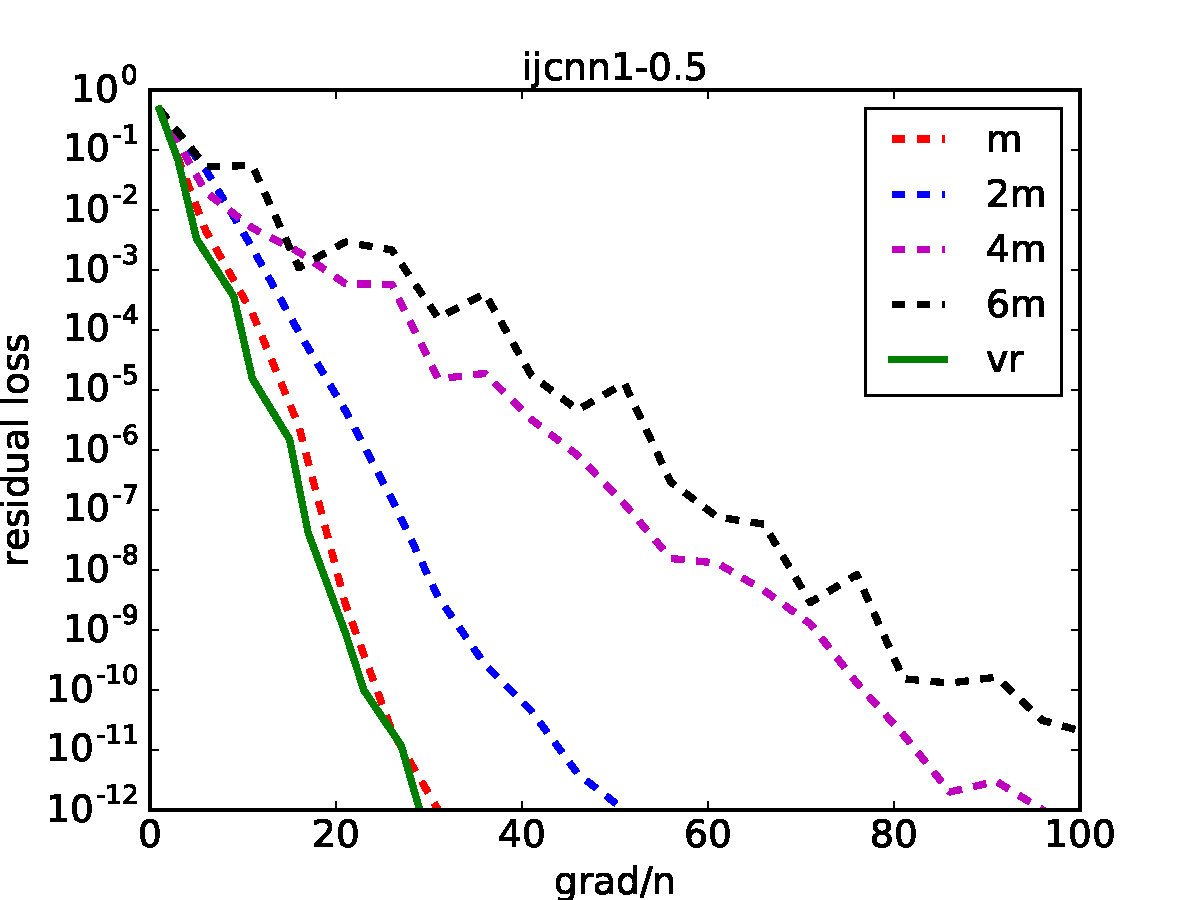
\includegraphics[width=0.24\linewidth]{ijcnn105}\label{ijcnn105}}
\subfigure[ijcnn1 $\eta=0.05$]{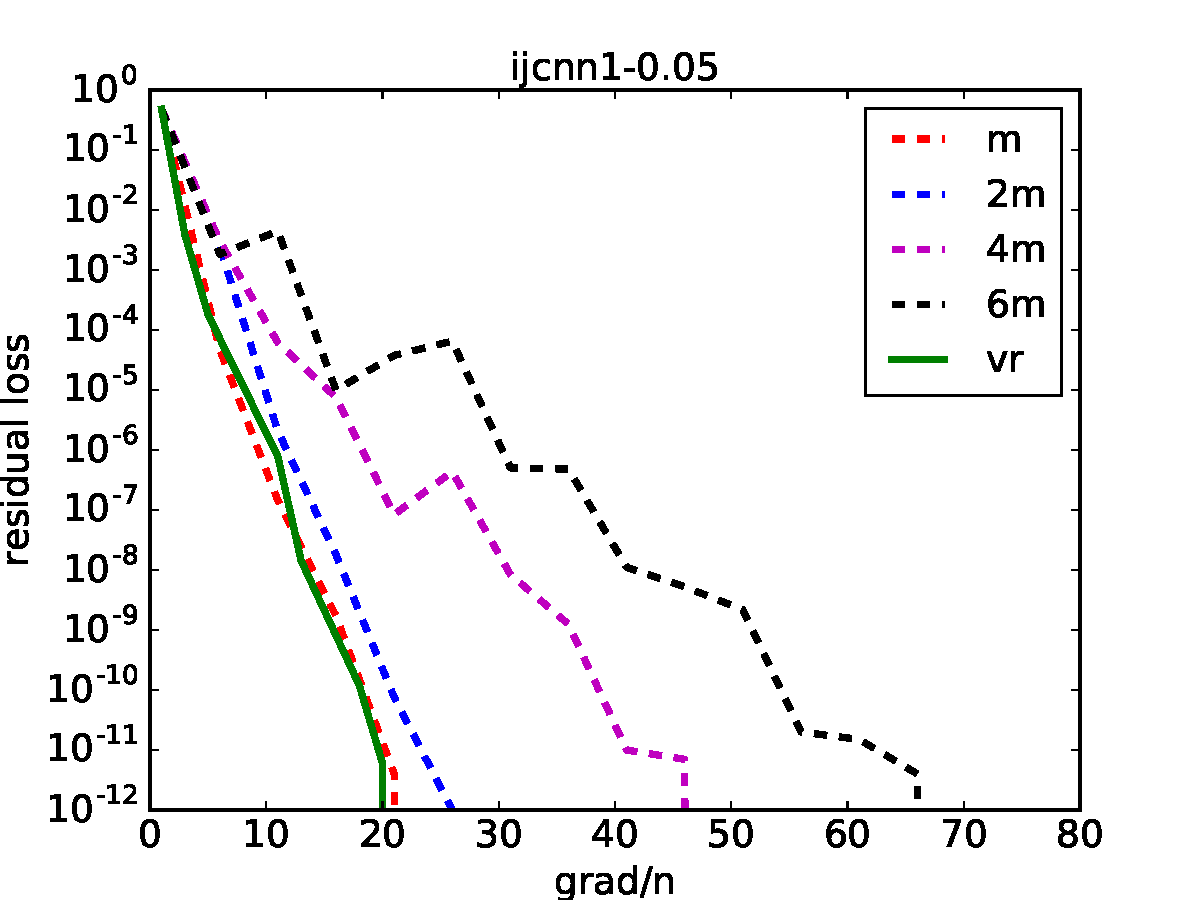
\includegraphics[width=0.24\linewidth]{ijcnn1005}\label{ijcnn1005}}
\subfigure[ijcnn1 $\eta=0.01$]{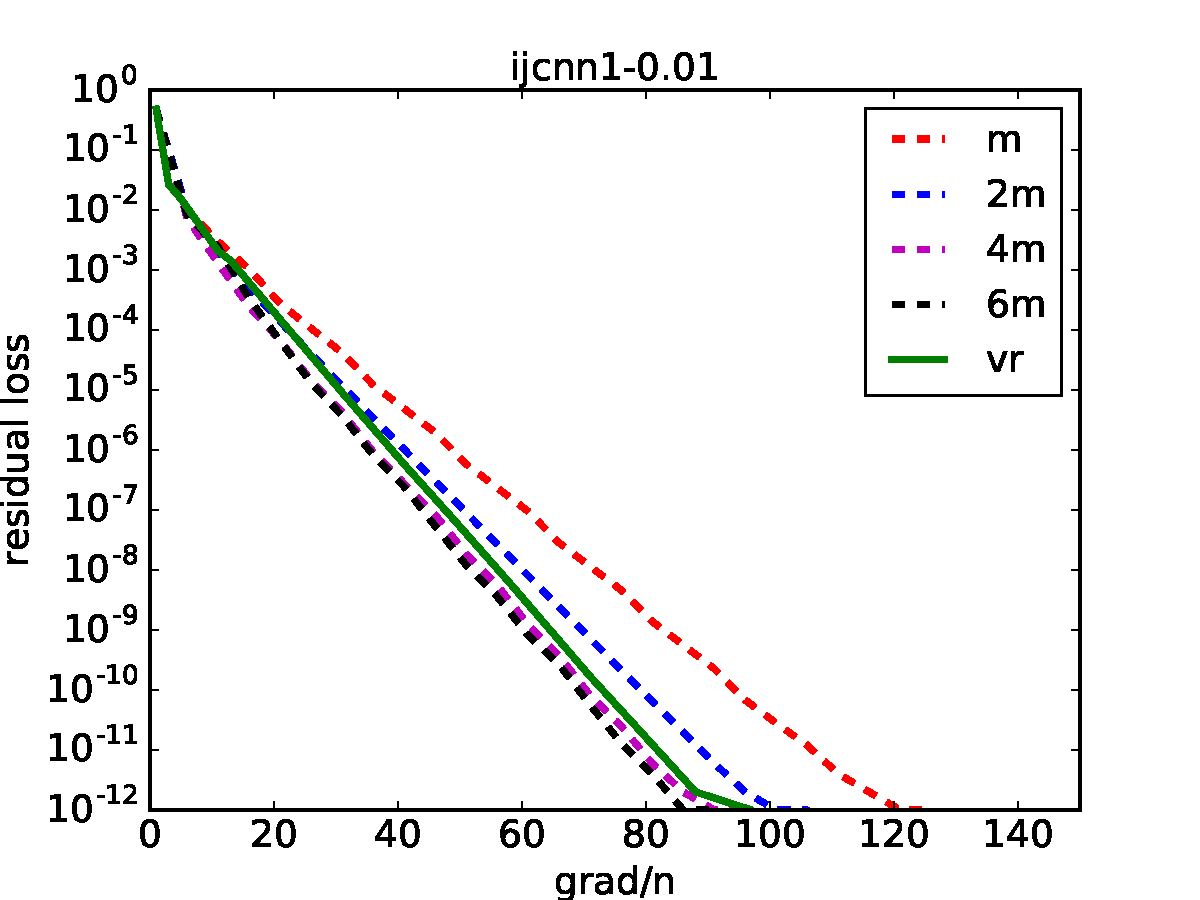
\includegraphics[width=0.24\linewidth]{ijcnn1001}\label{ijcnn1001}}
\subfigure[ijcnn1 $\eta=0.001$]{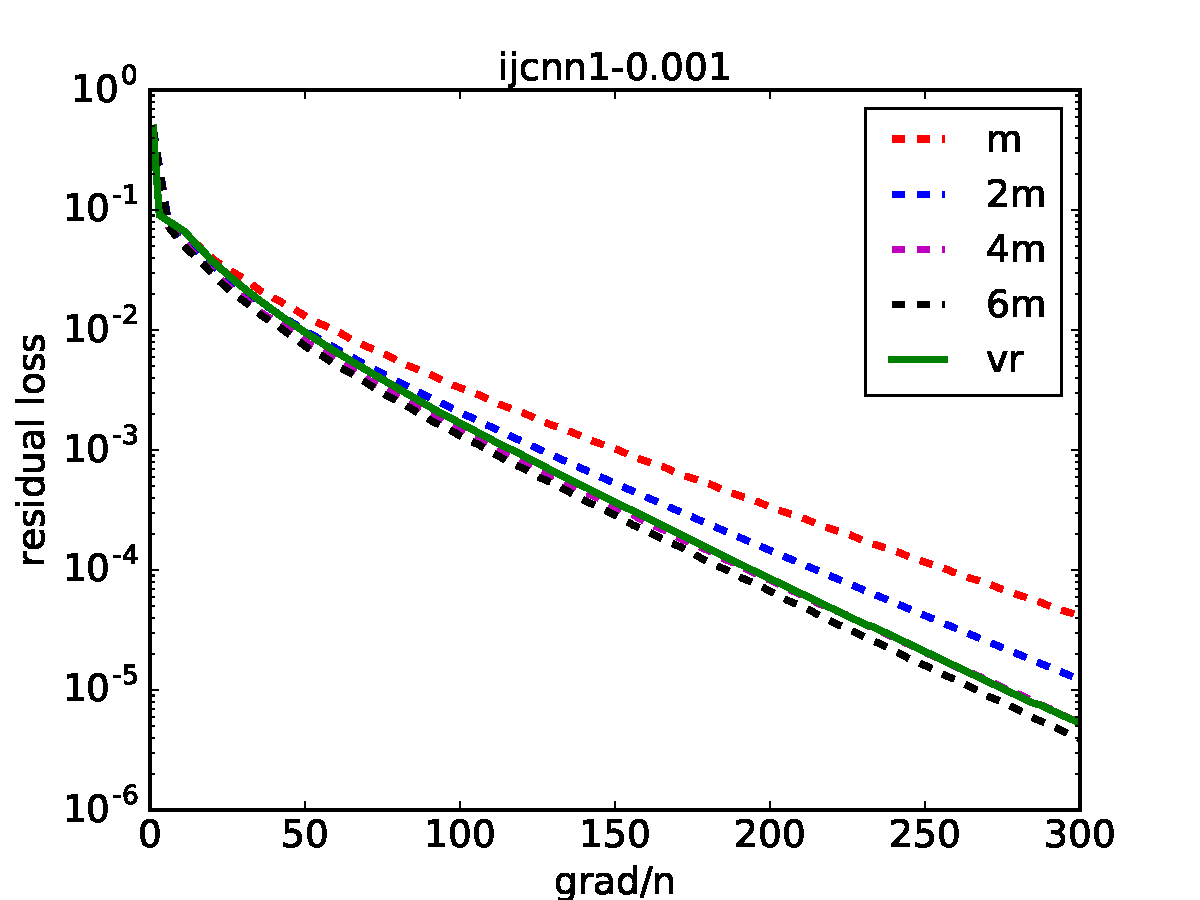
\includegraphics[width=0.24\linewidth]{ijcnn10001}\label{ijcnn10001}}

\subfigure[a9a $\eta=0.3$]{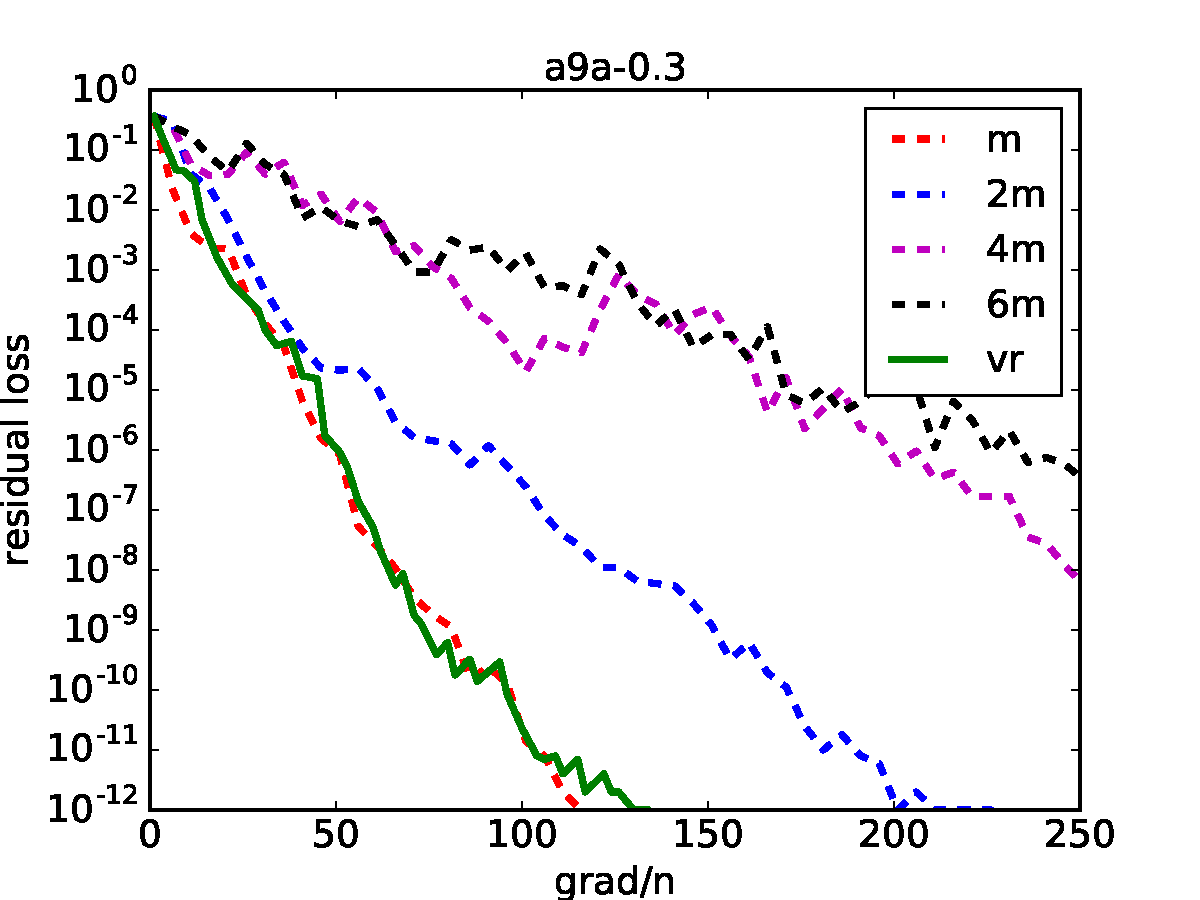
\includegraphics[width=0.24\linewidth]{a9a03}\label{a9a03}}
\subfigure[a9a $\eta=0.05$]{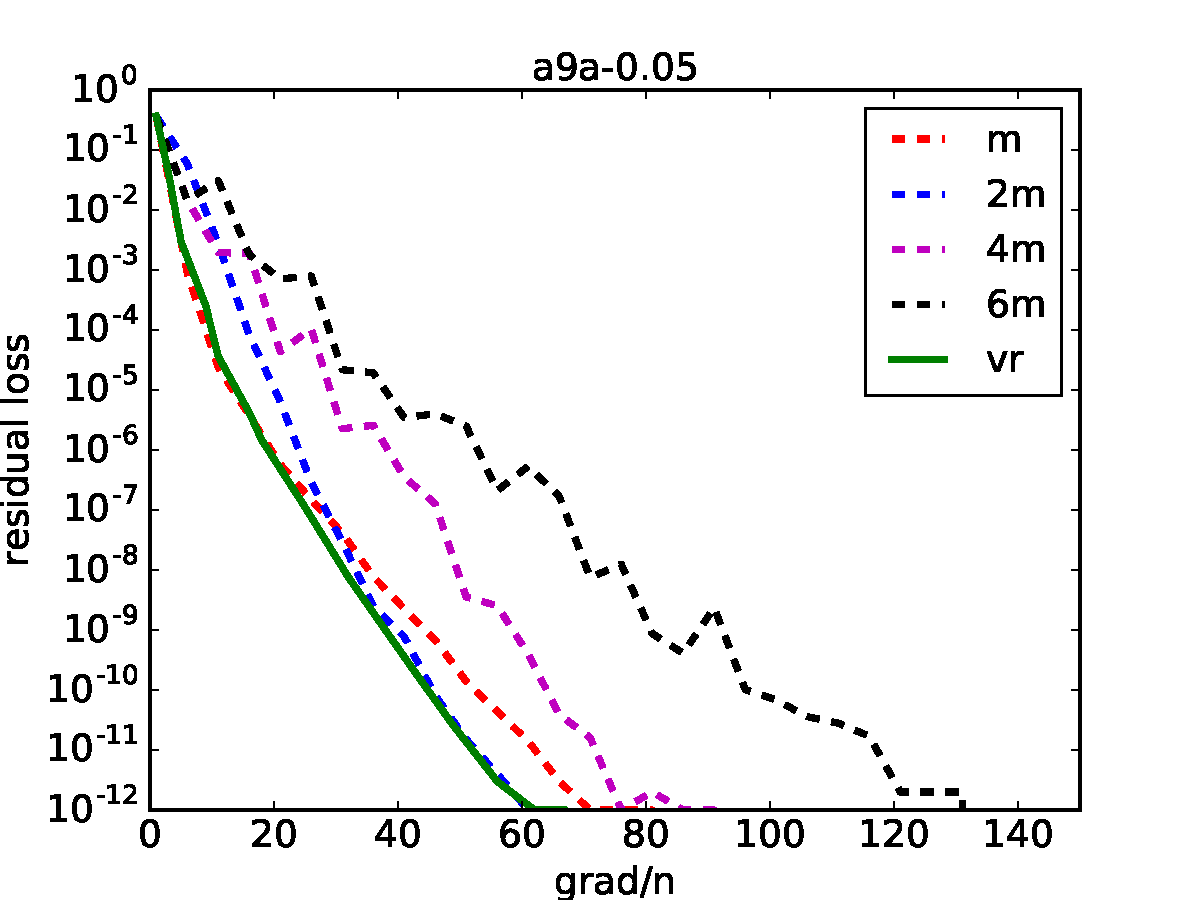
\includegraphics[width=0.24\linewidth]{a9a005}\label{a9a005}}
\subfigure[a9a $\eta=0.02$]{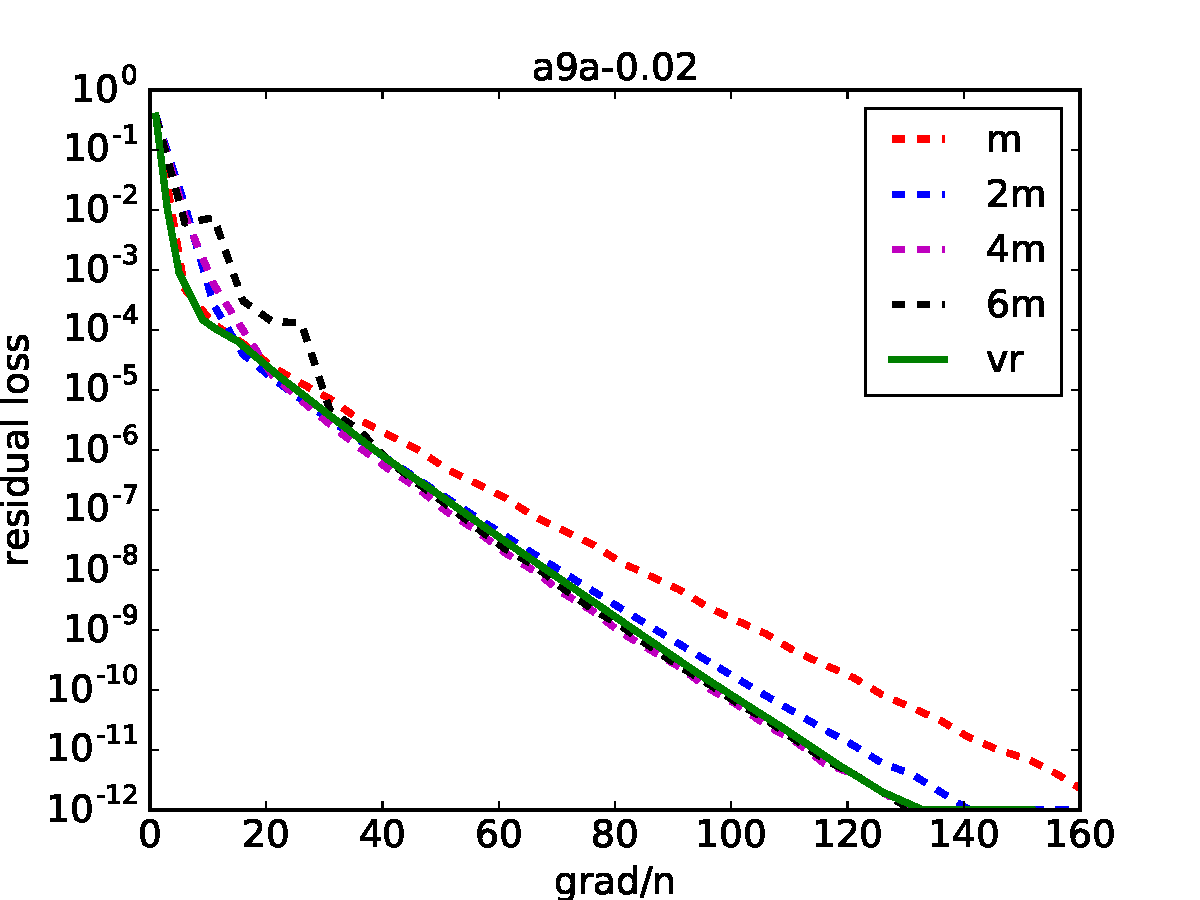
\includegraphics[width=0.24\linewidth]{a9a002}\label{a9a002}}
\subfigure[a9a $\eta=0.001$]{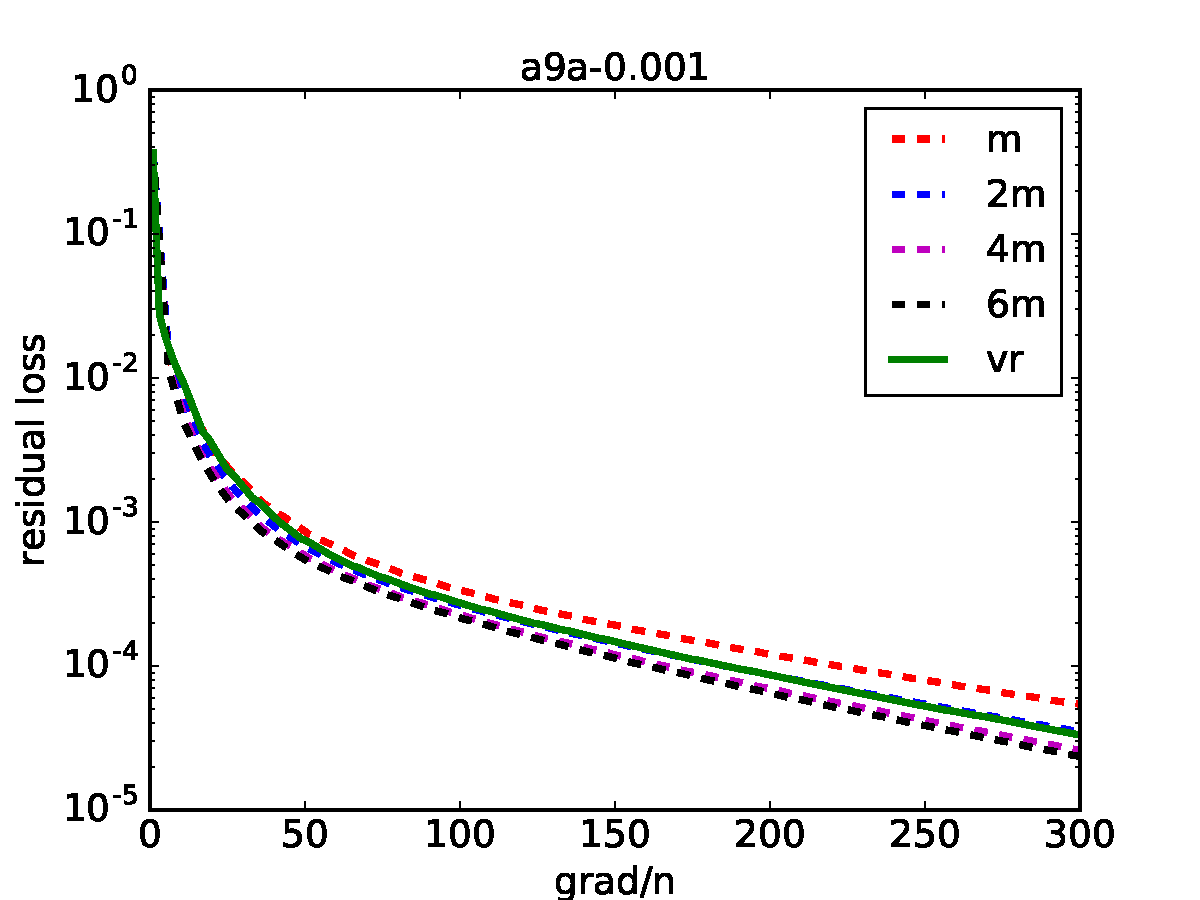
\includegraphics[width=0.24\linewidth]{a9a0001}\label{a9a0001}}
\subfigure[cpusmall $\eta=0.05$]{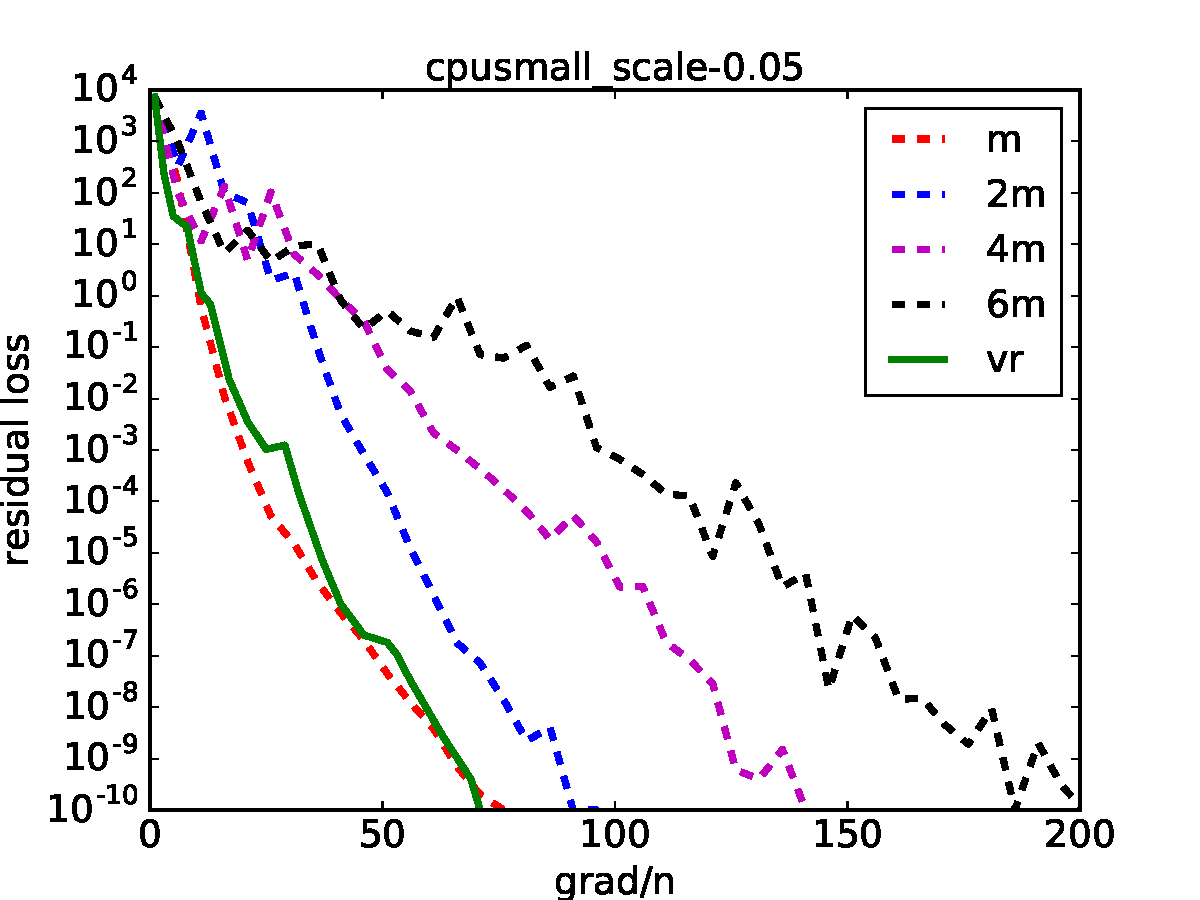
\includegraphics[width=0.24\linewidth]{cpusmall_scale005}\label{cpusmall_scale005}}
\subfigure[cpusmall $\eta=0.02$]{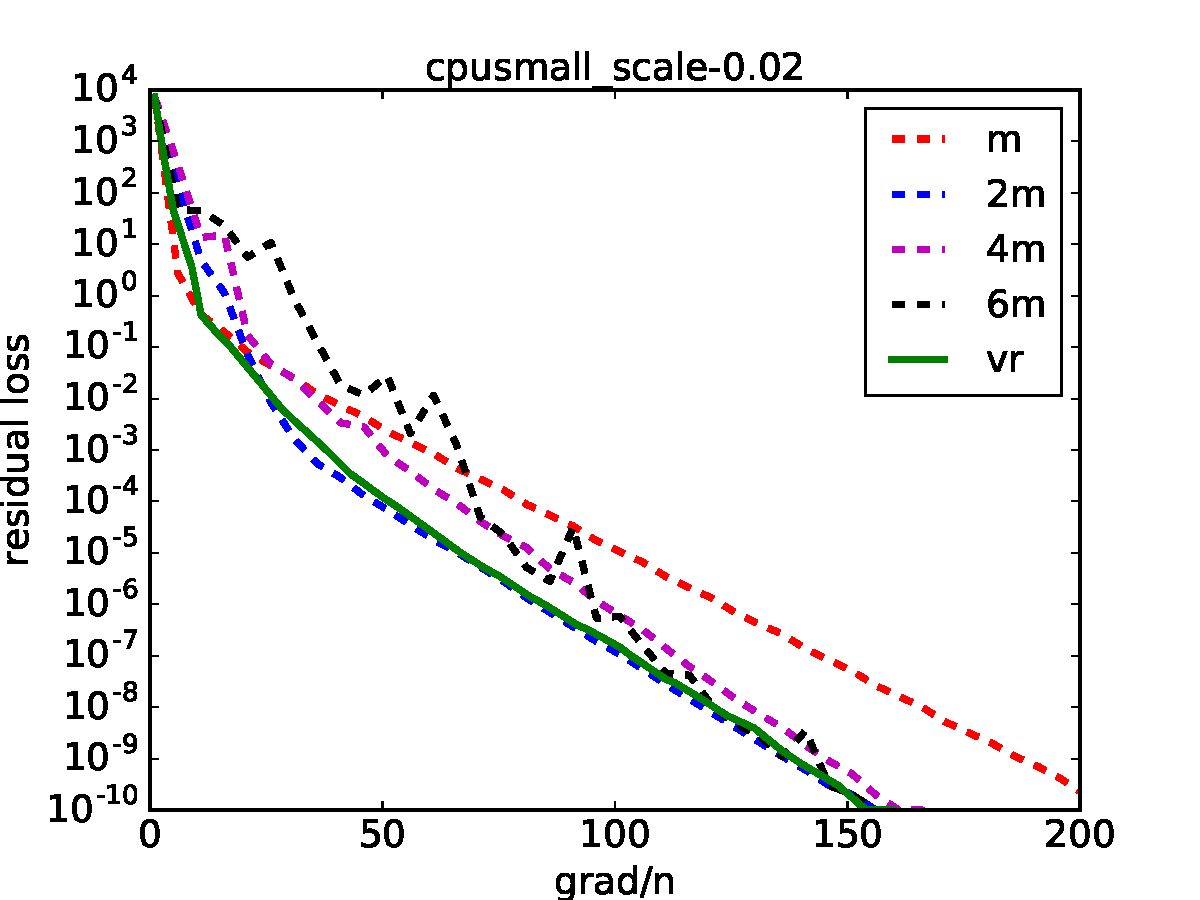
\includegraphics[width=0.24\linewidth]{cpusmall_scale002}\label{cpusmall_scale002}}
\subfigure[cpusmall $\eta=0.01$]{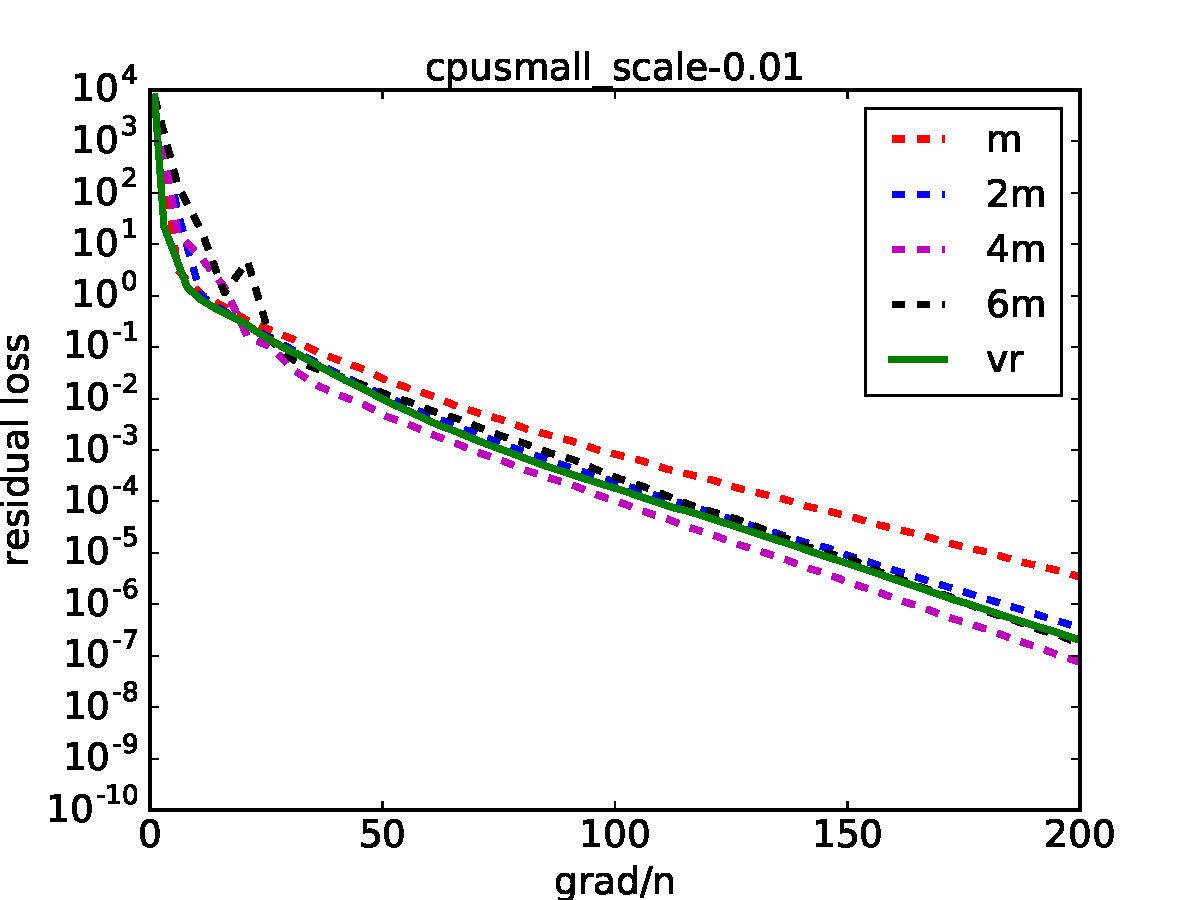
\includegraphics[width=0.24\linewidth]{cpusmall_scale001}\label{cpusmall_scale001}}
\subfigure[cpusmall $\eta=0.001$]{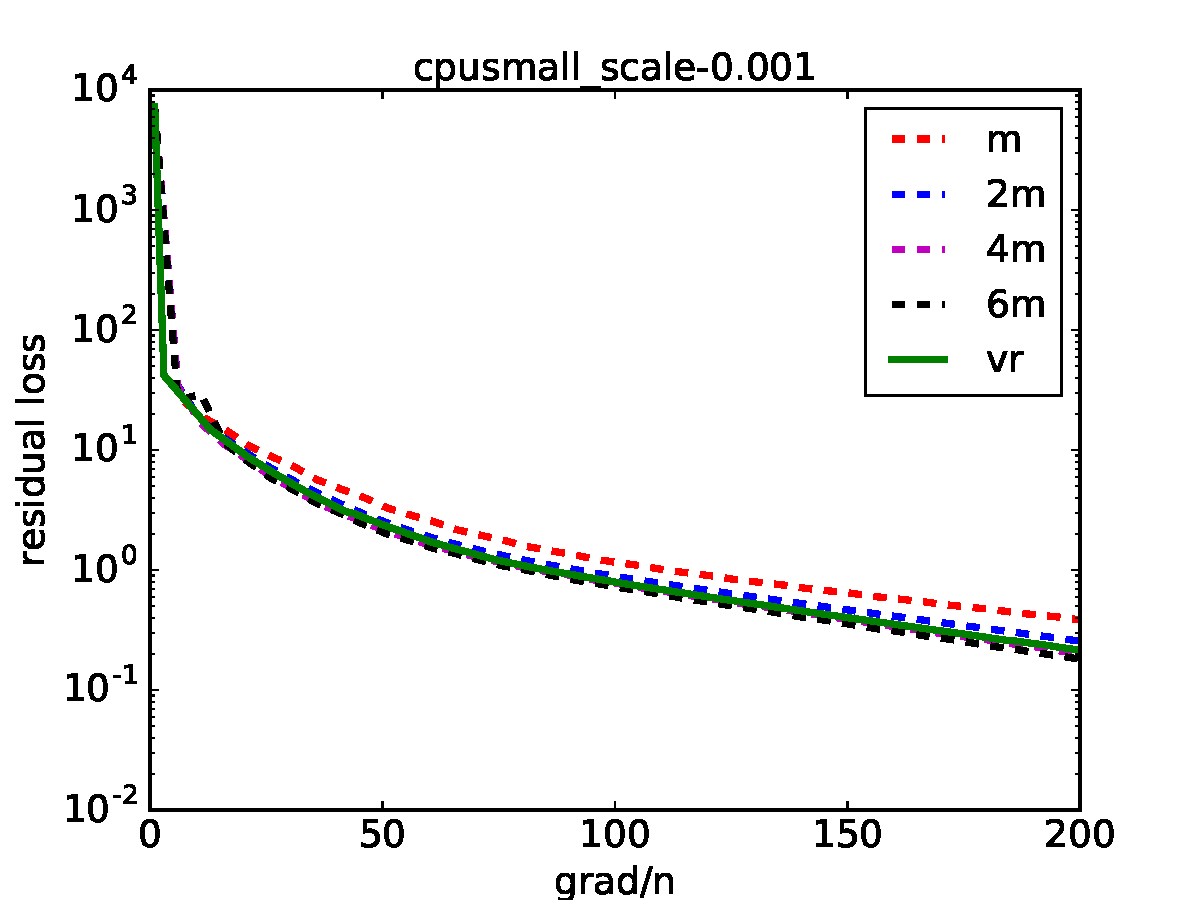
\includegraphics[width=0.24\linewidth]{cpusmall_scale0001}\label{cpusmall_scale0001}}
\subfigure[mg $\eta=0.1$]{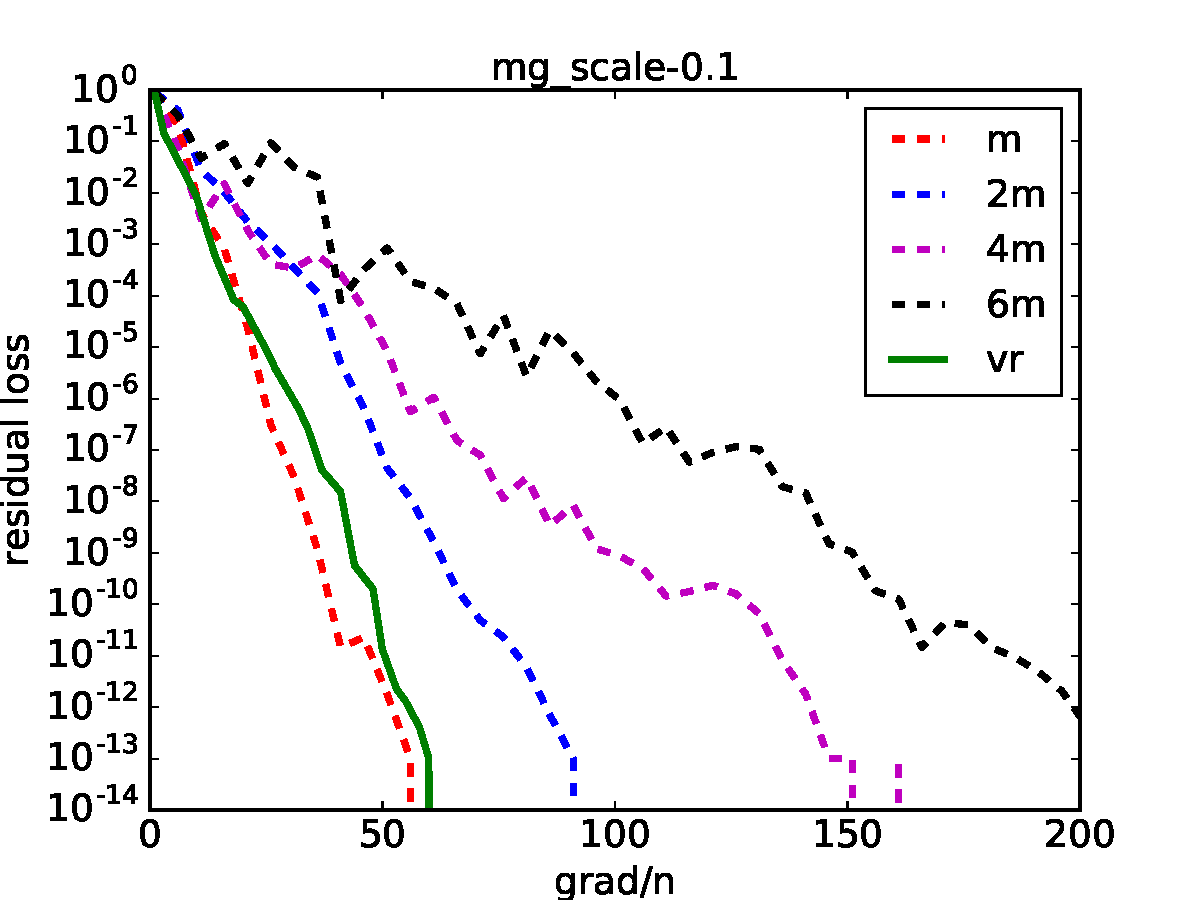
\includegraphics[width=0.24\linewidth]{mg_scale01}\label{mg_scale01}}
\subfigure[mg $\eta=0.01$]{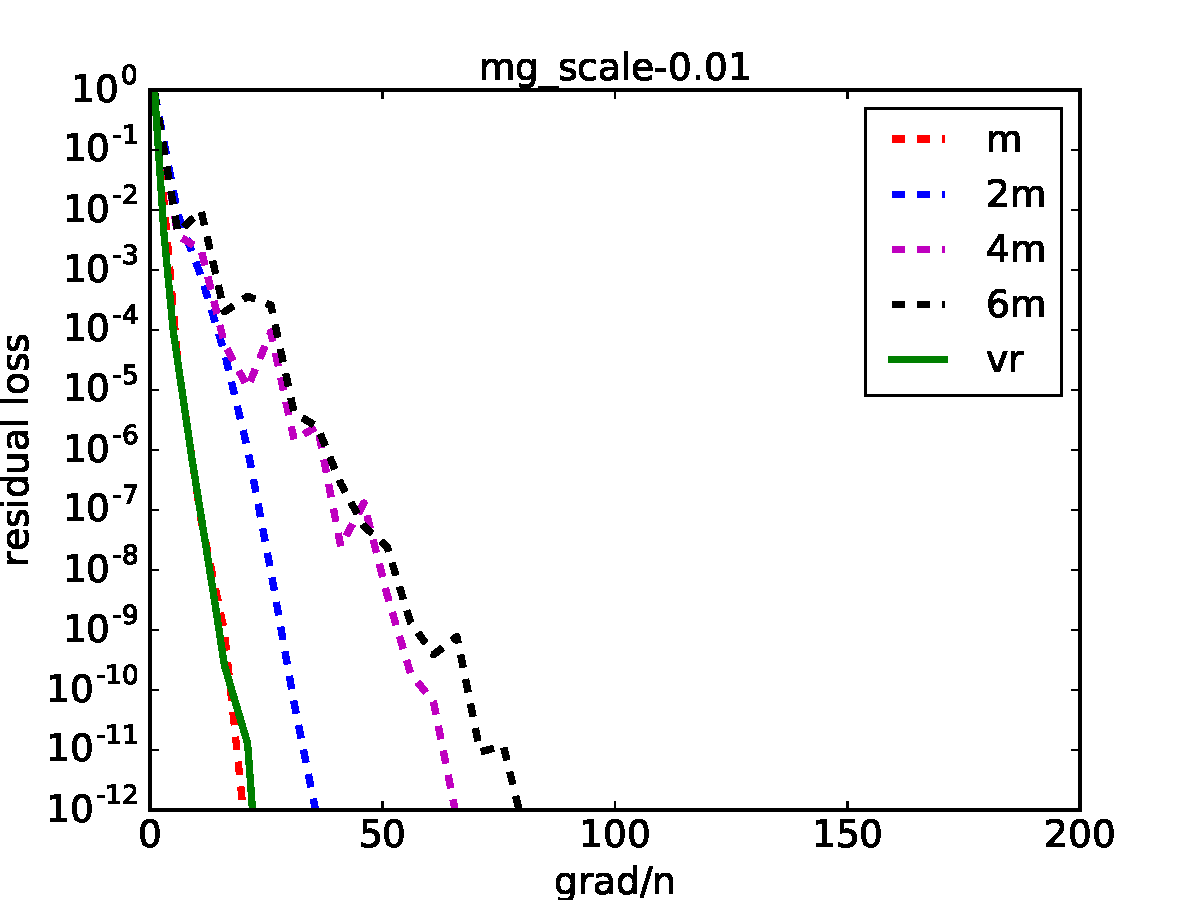
\includegraphics[width=0.24\linewidth]{mg_scale001}\label{mg_scale01}}
\subfigure[mg $\eta=0.005$]{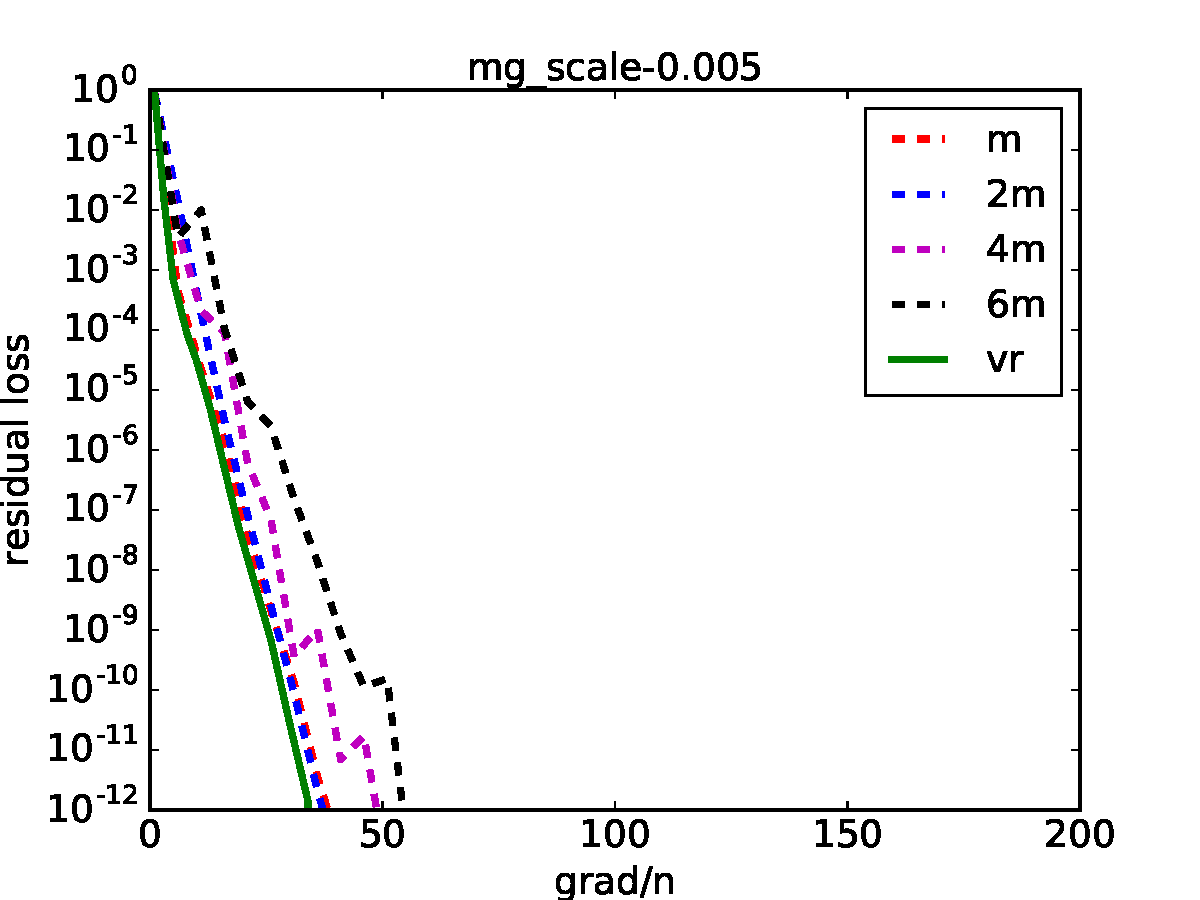
\includegraphics[width=0.24\linewidth]{mg_scale0005}\label{mg_scale0005}}
\subfigure[mg $\eta=0.001$]{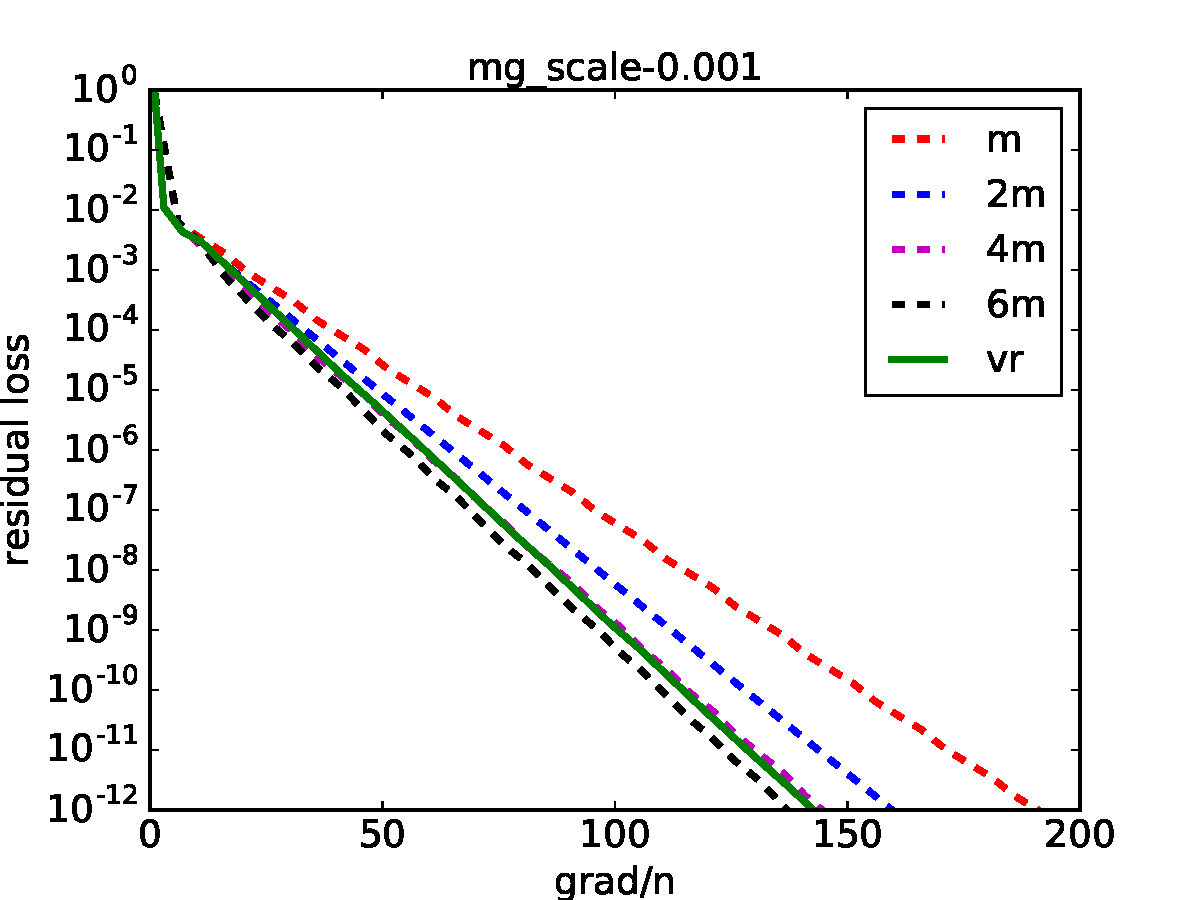
\includegraphics[width=0.24\linewidth]{mg_scale0001}\label{mg_scale0001}}
\label{figure_logistic_regression_convergence}
\caption{\textsc{scSVRG} can automatically set a appropriate $m$ for different learning rates}
\end{figure*}



 
\end{document}